\documentclass{beamer}

\usepackage{xspace}
\usepackage{tikz}
\usetikzlibrary{shapes,arrows}

\newcommand\javaPlex{\textsc{javaPlex}\xspace}
\newcommand\jPlex{\textsc{jPlex}\xspace}
\newcommand\Plex{\textsc{Plex}\xspace}

\begin{document}

\author{Andrew Tausz \and Mikael Vejdemo-Johansson}
\title{javaPlex -- persistent homology in Java}

\frame{\titlepage}

\begin{frame}
  \frametitle{Persistent homology}
  
  In a large variety of areas we encounter the following fundamental problem:

  \begin{block}{Problem}
    Estimate topological features of a shape based on a family of sample points (\emph{point clouds}).
  \end{block}
\end{frame}

\begin{frame}
  \frametitle{Persistent homology}
  
  Our favourite solution is due to Edelsbrunner, Letscher and Zomorodian.

  \begin{block}{Solution}
    \v Cech complexes, Vietoris-Rips complexes, $\alpha$-shapes and several other constructions capture by a filtered simplicial complex stemming from intersection relations of disks centered on the sample points

    \emph{Persistent homology} tracks the changes in topological features, and picks out such features that remain present over a long time.
  \end{block}
\end{frame}

\begin{frame}
  \frametitle{Persistent homology}
  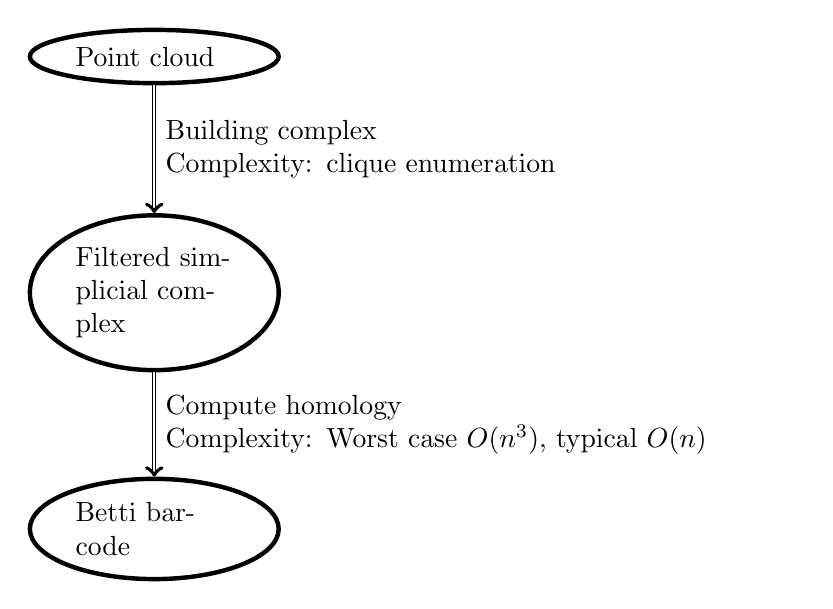
\begin{tikzpicture}[nodes={draw, ultra thick},node distance=3cm,text width=2cm]
    \node [ellipse] (pc) {Point cloud};
    \node [ellipse] (sc) [below of=pc] {Filtered simplicial complex};
    \node [ellipse] (bc) [below of=sc] {Betti barcode};
    \draw [->,double] (pc) -- node [right,draw=none,text width=8cm] {Building complex\\ Complexity: clique enumeration} (sc);
    \draw [->,double] (sc) -- node [right,draw=none,text width=8cm] {Compute homology\\ Complexity: Worst case $O(n^3)$, typical $O(n)$} (bc);
 \end{tikzpicture}
\end{frame}

\begin{frame}
  \frametitle{History of \Plex}
  
  Early developments in the theory of persistent homology took place at Stanford, as did the development of software to compute with point clouds.

  \begin{enumerate}
  \item \Plex \only<2>{-- C++, Matlab through MEX, memory hog}
  \item \jPlex \only<2>{-- Java, Matlab natively, BeanShell, highly optimized}
  \end{enumerate}
\end{frame}

\begin{frame}
  \frametitle{Design properties for \javaPlex}
  
  \javaPlex grew out of dissatisfaction with both \Plex and \jPlex.

  \begin{block}{Disadvantages}
    \begin{columns}[t]
      \begin{column}{0.5\textwidth}
        \Plex
        \begin{itemize}
        \item Dependent on exact Matlab version and \textsc{mex} dialect
        \item Design carrying \emph{very} many pointers: high memory consumption
        \end{itemize}
      \end{column}
      \begin{column}{0.5\textwidth}
        \jPlex
        \begin{itemize}
        \item Too highly optimized: no real capacity to extend or modify
        \item Not actually competitive enough to motivate this
        \end{itemize}
      \end{column}
    \end{columns}
  \end{block}
\end{frame}

\begin{frame}
  \frametitle{Usage examples}
  
\end{frame}




\end{document}

%%% Local Variables: 
%%% mode: latex
%%% TeX-master: t
%%% End: 
